\section*{Introduction}
Dans ce chapitre, nous expliquerons en détails les méthodes que nous avons employées pour l’ADT.\\
Pour commencer, nous exposerons une description de la notation de la batterie ainsi qu’une modélisation de celle-ci pour la représentation des données rythmiques en arbres syntaxiques. Nous poursuiverons avec une présentation de qparse\footnote{https://qparse.gitlabpages.inria.fr/}, un outil de transcription qui est développé par Florent Jacquemard (Inria) au sein du laboratoire Cedric au CNAM.\\
Enfin, nous présenterons les systèmes. 
\section{La notation de la batterie}
\begin{figure}[h]
	\centering
	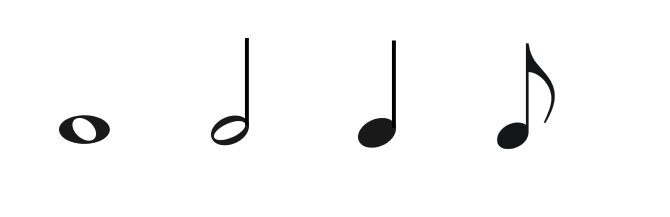
\includegraphics[height=10mm, width=25mm]{z_images/3_methodes/0_notation_de_la_batterie/0_figures_de_notes.png}
\end{figure}
Une figure de note \cite{danhauser} de musique réunit plusieurs critères\footnote{\url{https://fr.wikipedia.org/wiki/Note_de_musique}} :
\begin{itemize}
	\item Une tête de note :\\
	Sa position sur la portée indique la hauteur de la note. La tête de note peut aussi indiquer une durée.
	\item Une hampe :\\
	Indicatrice d’appartenance à une voix en fonction de sa direction et indicatrice d’une durée représentée par sa présence ou non (blanche ≠ ronde)
	\item Un crochet : La durée d’une note est divisée par deux à chaque crochet ajouté à la hampe d’une figure de note.
\end{itemize}
\begin{figure}[h]
	\centering
	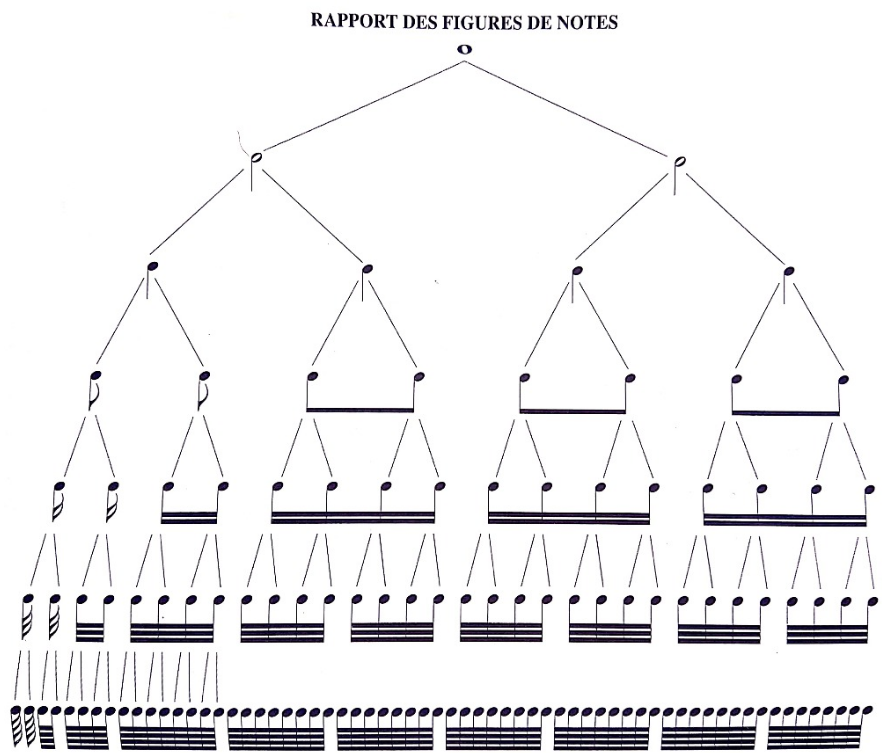
\includegraphics[height=50mm, width=80mm]{z_images/3_methodes/0_notation_de_la_batterie/1_rapport_figures_notes.png}
	\caption{Rapport des figures de notes}\cite{danhauser}
	\label{rapp_fig_notes}
\end{figure}
La figure \ref{rapp_fig_notes} montre les rapports de durée entre les figures de notes. Plus les durées sont longues, plus elles sont marquées par la tête de note (la note carrée fait deux fois la durée d’une ronde) ou la présence ou non de la hampe. À partir de la noire (3ème lignes en partant du haut), on ajoute un crochet à la hampe d’une figure de notes pour diviser sa durée par 2. Les notes à crochet (croche , double-croche, triple…) peuvent être reliées ou non par des ligatures (Voir les 4 dernière lignes de la figure \ref{rapp_fig_notes}).
\subsection*{Les hauteurs et les têtes de notes}
Pour la transcriptions, nous proposons une notation inspirée du recueil de pièces pour batterie de J.-F. Juskowiak \cite{jusko} et des méthodes de batterie Agostini \cite{ago_meth_3}, car nous trouvons la position des éléments cohérente et intuitive.\\
En effet, les hauteurs sur la portée représentent :
\begin{itemize}
	\item La hauteur physique des instruments :\\
	La caisse claire est centrale sur la portée et sur la batterie (au niveau de la ceinture, elle conditionne l’écart entre les pédales et aussi la position de tous les instruments basiques d’une batterie).\\
	Tous ce qui en dessous de la caisse-claire sur la portée est en dessous de la caisse-claire sur la batterie (pédales, tom basse) ;\\
	Tous ce qui est au dessus de la caisse-claire sur la portée, l’est aussi sur la batterie.\\
	\item La hauteur des instruments en terme de fréquences :\\
	Sauf pour le charley au pied et si l’on sépare en trois groupes (gc, toms, cymbales), de bas en haut, les instruments vont dans du plus grave au plus aigu.
\end{itemize}
\begin{figure}[!h]
	\centering
	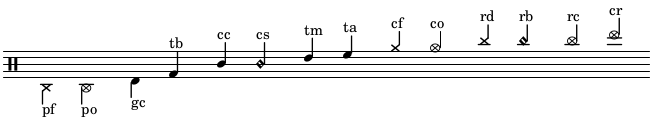
\includegraphics[height=25mm, width=130mm]{z_images/3_methodes/0_notation_de_la_batterie/2_hauteurs_et_tete_de_notes.png}
	\caption{Hauteur et têtes de notes}
	\label{Hauteur et têtes de notes}
\end{figure}
Les noms des instruments correspondant aux codes des notes de la figure \ref{Hauteur et têtes de notes} sont dans le tableau \ref{Pitchs et instruments}.
\subsection*{Les durées}
\label{hho}
Comme nous venons de la voir, la majorité des instruments de la batterie sont représentés par les têtes des notes. Par conséquent, l’usage des symboles rythmiques concernant la tête de note ne pourront pas être utilisées. Ceci est valable aussi pour la présence ou non de la hampe puisque ce phénomène n’existe qu’avec les têtes de notes de type cercle-vide (opposition blanche-ronde). L’usage des blanches existe dans certaines partitions de batterie [ref??system drum ou rythmique bin n.1] mais celà reste des cas très rares. Certains logiciels permettent de faire des blanches avec des symboles spécifiques à la batterie ou aux percussions mais leur lecture reste peu aisée et leur utilisation pour la batterie est rarissime également.\\
La durée d’une note peut être allongée par divers symboles :
\begin{itemize}
	\item Le point ;
	\item La liaison.
\end{itemize}
Ces symboles ne seront utiles que pour l’écriture des ouvertures de charley. Le charley est le seul instrument de la batterie dont la durée est quantitifiée (les cymbales attrapées à la main peuvent l’être aussi mais cela est très rare.)\newpage
\begin{figure}[h]
	\centering
	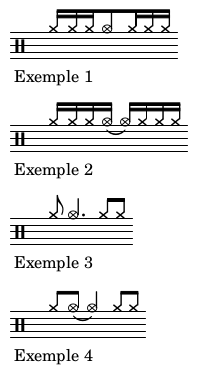
\includegraphics[height=80mm, width=40mm]{z_images/3_methodes/0_notation_de_la_batterie/3_point_et_liaison.png}
	\caption{Point et liaison}
	\label{point_liaison}
\end{figure}
L’écriture de la batterie doit faire ressortir la pulsation. La première chose à prendre en compte pour analyser la figure \ref{point_liaison} est donc la nécessité de regrouper les notes par temps à l’aide des ligatures.\\
exemple 1 : ouverture de charley quantifiée mais pas notes pas regroupées par temps.\\
exemple 2 : bieeen !\\
exemple 3 et exemple 4 : les deux exemples sont valables mais le deuxième est le plus souvent utilisé car plus intuitif (regroupement par temps).\\
En cas de nécéssité de rallonger la durée d’une note pour la batterie, on privilégiera la liaison.
\subsection*{Les silences}
\begin{figure}[h]
	\centering
	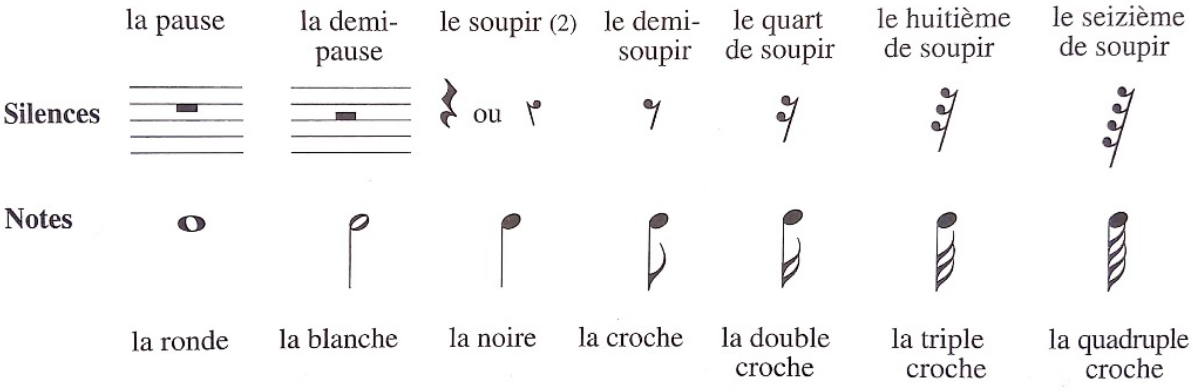
\includegraphics[height=40mm, width=125mm]{z_images/3_methodes/0_notation_de_la_batterie/4_silences.png}
	\caption{Les silences}
	\label{silences}
\end{figure}
Les silences sont parfois utilisées pour quantifier les ouvertures de charley. Les fermetures du charley sont notées soit par un silence (correspondant à une fermeture de la pédale), soit par un écrasement de l’ouverture par un autre coup de charley fermé, au pied ou à la main.
Physiquement, le charley est fermé par une pression du pied sur la pédale de charley. Dans les fichiers MIDI, cette pression est traduite par un charley joué au pied. Mais dans une vraie partition, cette écriture ne traduirait pas ce que le batteur doit penser.
\begin{figure}[h]
	\centering
	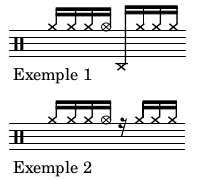
\includegraphics[height=40mm, width=40mm]{z_images/3_methodes/0_notation_de_la_batterie/5_silence_joue.png}
	\caption{Silence joué}
	\label{silence joue}
\end{figure}\\
L’exemple 1 de la figure \ref{silence joue} montre ce qui est écrit dans les données MIDI et l’exemple 2 montre ce que le batteur doit penser en lisant la partition. Il faut aussi prendre en compte l’écriture surchargée que l’exemple 1 donnerait avec une partition comprenant plusieurs voix et plusieurs instruments jouant simultanément.
\subsection*{Les équivalences rythmiques}
Pour les instruments mélodiques, la liaison et le point sont les deux seules possibilités en cas d’équivalence rythmique pour des notes dont la durée de l’une à l’autre est ininterrompue. Mais pour la batterie, à part pour les ouvertures de charley (voir section \ref{hho}), les durées des notes n’ont pas d’importance. L’usage des silences pour combler la distance rythmique entre deux notes devient donc possible.\\
Ceci pris en compte, et étant donné que les indications de durée dans les têtes de notes sont peu recommandées (voir section \ref{hho}), l’écriture à l’aide de silences sera privilégiée comme indication de durée sauf dans les cas où cela reste impossible. Ce choix à pour but de n’avoir qu’une manière d’écrire toutes les notes, que leurs têtes de notes soit modifiées ou non.
\begin{figure}[h]
	\centering
	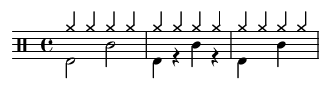
\includegraphics[height=20mm, width=75mm]{z_images/3_methodes/0_notation_de_la_batterie/6_equivalence.png}
	\caption{Équivalence}
	\label{equivalence}
\end{figure}\\
Sur la figure \ref{equivalence}, théoriquement, il faudra choisir la notation de la deuxième mesure mais dans certains contexte, pour des raisons de lisibilité ou de surcharge, la version sans les silences de la troisième mesure pourra être choisie.
\subsection*{Les voix}
Les voix\footnote{\url{https://fr.wikipedia.org/wiki/Voix_(polyphonie)}} désignent les différentes parties mélodiques constituant une composition musicale et destinées à être interprétées, simultanément ou successivement, par un ou plusieurs musiciens. En batterie, une voix regroupe par les ligatures les instruments qui, à eux seuls constituent une phrase rythmique. Plusieurs écritures étant possibles pour un même rythme. On peut regrouper les instruments de la batterie par voix. Sur une portée de batterie, il existe le plus souvent 1 ou 2 voix. Sur la figure \ref{sep_voix}, il faudra faire un choix entre les exemples 1, 2 et 3 qui sont trois façons d’écrire le même rythme.
\begin{figure}[h]
	\centering
	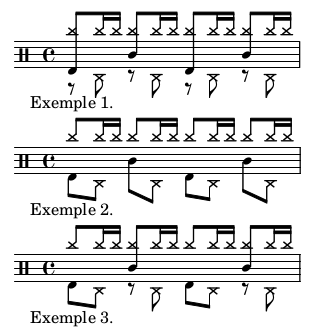
\includegraphics[height=65mm, width=60mm]{z_images/3_methodes/0_notation_de_la_batterie/7_voix.png}
	\caption{Séparation des voix}
	\label{sep_voix}
\end{figure}\\
Ce choix se fera en fonction des instruments joués, de la nature plus ou moins systèmatique de leurs phrasés, et des associations logiques entre les instruments dans la distribution des rythmes sur la batterie.\\
%Ainsi l’arbre syntaxique de départ sera divisé en autant d’instruments qui le constituent et les voix seront regroupées de manière cohérentes.
\subsection*{Les accentuations et les ghost-notes}
a = accent\\
g = ghost-note\\
$\Rightarrow$ nuance ≠ accentuation
\begin{figure}[h]
	\centering
	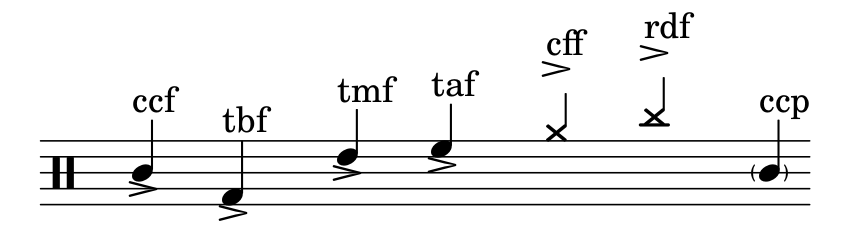
\includegraphics[height=25mm, width=75mm]{z_images/3_methodes/0_notation_de_la_batterie/8_nuances_0.png}
	\caption{Les nuances}
	\label{nuances}
\end{figure}\\
La figure \ref{nuances} ne prend en compte que les accents que nous avons estimé nécessaires. En effet, les nuances jouées avec les pieds ne sont pas significatives, certaines vélocités en dessous de 40 n’étant détectées et inscrites dans les données MIDI sont dû au mouvement du talon du batteur perçu par le capteur mais pas jouées intentionnellement.
\begin{figure}[h]
	\centering
	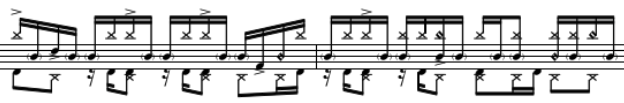
\includegraphics[height=20mm, width=110mm]{z_images/3_methodes/0_notation_de_la_batterie/8_nuances_1.png}
	\caption{Exemple pour les nuances}
	\label{exemple_nuances}
\end{figure}
\section{Modélisation pour la transcription}
\label{modelisation_transcription}
\subsection*{Les pitchs}
\begin{table}[h]
	\centering
	\begin{tabular}{|c|c|c|} \hline
		Codes & Instruments & Pitchs \\ \hline
		cf & charley-main-fermé & 22, 42 \\
		co & charley-main-ouvert & 26 \\
		pf & charley-pied-fermé & 44 \\
		rd & ride & 51 \\
		rb & ride-cloche (bell) & 53 \\
		rc & ride-crash & 59 \\
		cr & crash & 55 \\
		cc & caisse-claire & 38, 40 \\
		cs & cross-stick & 37 \\
		ta & tom-alto & 48, 50 \\
		tm & tom-medium & 45, 47 \\
		tb & tom-basse & 43, 58 \\
		gc & grosse-caisse & 36 \\ \hline
	\end{tabular}
	\caption{Pitchs et instruments}
	\label{pitchs_instru}
\end{table}
Un large panel d’instruments sont disponibles pour chaque instrument basique de la batterie. Pour cette première version, les instruments basiques de la batterie ont été conservés comme réceptacle pour tous les différents intruments qui rentrent dans leur catégorie, c’est pourquoi certain code-instrument se voit attribuer plusieurs pitchs dans tableau \ref{pitchs_instru}.
Il semblerait qu’aucun pitch ne désigne le charley pied ouvert…
\subsection*{La vélocité}
\label{velocite}
\begin{table}[h]
	\centering
	\begin{tabular}{|c|c|c|c|} \hline
		Codes & Instruments & Pitchs & Vélocité \\ \hline
		cop & charley-main-ouvert & 46 & ? \\ \hline
	\end{tabular}
	\caption{Vélocité et nuances}
\end{table}
Nous ne prendrons en compte la vélocité que pour la cc, les toms et les cymbales jouées aux mains. Les nuances de grosse caisse et charley aux pieds sont le plus souvent insignifiantes, elles ne sont marquées sur le figure qu’à titre indicatif.
Si la vélocité est en dessous de 40, il s’agit de ghost-notes : la tête de note devra être entouré de parenthèses et le suffixe \textit{p (piano)} devra être ajouté au codes de l’instrument. (Voir ccp ci-dessus.)
Si la vélocité est au dessus de 90, il s’agit de notes accentuées : le symbole « > » et le suffixe \textit{f (forte)} devra être ajouté au codes de l’instrument. (Voir ccf ci-dessus.)
Lorsque la vélocité va de 40 à 89, on considèrera le volume comme normal et aucun symbole supplémentaire ne sera ajouté à la note.\\\\

%\subsubsection{Les dilemmes}
Le charley de pitch 46 est considéré comme le charley ouvert joué à la main sur le haut de la cymbale mais souvent, ça correspond au geste « tranche-olive » de la baguette lorsque le batteur accentue avec la tranche et joue moins fort avec l’olive sur le plat de la cymbale. Je vais dans un premier temps considérer le pitch comme \textbf{charley-main-ouvert-piano} (ghost-note)
\subsection*{Les arbres de rythmes}
Voici une représentation de la figure \ref{sep_voix} en arbre de rythme avec les codes de chaque instrument :\\\\
\Tree[ [ [rd\\gc ][ [rd\\pf ][rd ]]]
[ [rd\\cc ][ [rd\\pf ][rd ]]]
[ [rd\\gc ][ [rd\\pf ][rd ]]]
[ [rd\\cc ][ [rd\\pf ][rd ]]] ]\\\\\\
Ci-dessous, le même arbre dont les codes des instruments sont remplacés par leurs données midi respectives :\\\\
\Tree[ [ [51\\36 ][ [51\\44 ][51 ]]]
[ [51\\38 ][ [51\\44 ][51 ]]]
[ [51\\36 ][ [51\\44 ][51 ]]]
[ [51\\38 ][ [51\\44 ][51 ]]] ]\\\\\\
Cet arbre représente un rythme unique dont les possibilités de notation sur une partition sont théoriquement multiples. Les trois exemples de la figure 3.4 peuvent-être représentés par les arbres ci-dessus.
\section{Qparse}
Florent Jacquemard(Inria), Philippe Rigaux (CNAM), Masahiko Sakai (Nagoya U.), Francesco Foscarin (PhD, CNAM), Clement Poncelet (Salzburg U.)
\textit{Mettre ici un schéma de la chaîne de traitement de qparse (workflow)}\\
Pb du MIDI avec qparse entrée ON-OFF $\Rightarrow$ sortie 1 seul symbole.\\
Qparse produit une partition musicale en prenant en entrée une performance musicale symbolique (par exemple un fichier MIDI) et un automate à arbre pondéré décrivant un langage de rythmes préférés (grammaire pondérée). La quantification des rythmes est basée sur des algorithmes d’analyse syntaxique applicables sur des automates arborescents.\footnote{\url{https://qparse.gitlabpages.inria.fr}}
En entrée : midi (séquence d’événements datés (piano roll) accompagné d’une grammaire pondérée)\\
$\Rightarrow$ parsing\\
$\Rightarrow$ global parsing tree\\
$\Rightarrow$ RI (Représentation Intermédiaire) arbres locaux par intruments\\
$\Rightarrow$ Sortie (xml, mei, lilypond,… )\\
Minimiser la distance entre le midi et la représentation en arbre.\\
\textbf{Un des problèmes de Qparse était qu’il était limité au monophonique.}
$\Rightarrow$ \textit{Expliquer ici les limites du monophonique…}
%\subsection{Les Jams}
%Regroupement par nature des notes qui forment un accord.
\subsection*{La grammaire pondérée}
La grammaire pondérée qui accompagne le MIDI en input est une grammaire hors-contexte pondérée. Chaque règle comporte un poid qui sert à favoriser certains rythmes plutôt que d’autres.\footnote{\url{https://qparse.gitlabpages.inria.fr/docs/scientific/}}
\subsection*{Le parsing}
Le parsing du midi donné en input crée une représentation symbolique sous forme d’arbre de rythme.\\
Ici $\Rightarrow$ exemple avec :\\
3bars\_fill\_groove-016.mid $\Rightarrow$ arbre\\
\subsection*{La réécriture}
\subsubsection{Séparation des voix}
\subsubsection{Simplification}
Ici, description basique des règles de réécriture 
\section{Les systèmes}
\label{systemes_methodes}
Un système est la combinaison d’un ou plusieurs éléments qui jouent un rythme en boucle (motif) et d’un autre élément qui joue un texte rythmique variable mais respectant les règles propre au système (gamme).\\

Système = motif + gamme/texte\\
motif = rythmes coordonnés joués avec 2 ou 3 membres en boucle (reparti sur 1 ou 2 voix)\\
gamme/texte = rythme irrégulier joué avec un seul membre sur le motif (Réparti sur 1 voix). La gamme d’un système considère l’ensemble des combinaisons que le batteur pourrait rencontrer en interprétant un texte rythmique à l’aide du système.\\

Nous partirons de propositions génériques de systèmes (environs trois systèmes dans différents styles de batterie) que nous tenterons de détecter dans le jeu de données groove.\\

Quatre systèmes standards :
\begin{itemize}
	\item binaire
	\item ternaire (shuffle, afro, rock)
	\item jazz
	\item afro-cubain\\
\end{itemize}

Nous travaillerons aussi sur la détection de répétitions sur plusieurs mesures afin de pouvoir corriger des erreurs sur une des mesures qui aurait dû être identique aux autres mais qui présente des différences.

\subsubsection{Intérêt des systèmes}
\textit{\textbf{Détection d’indication de mesure et choix de grammaire pondérée}}\\
Il faut prendre en compte l’existence potentielle de plusieurs grammaires \textit{(un fichier wta par grammaire)} chacunes dédiées à un type de contenu MIDI. Le choix d’une grammaire pondérée doit être fait avant le parsing puisque qparse prends en entrée un fichier MIDI et un fichier wta.\\
Pour les expériences effectuées avec le Groove MIDI Data Set, le style et l’indication de mesure sont récupérables par les noms de fichiers MIDI, mais il faudra par la suite les trouver automatiquement sans autres indications que les données MIDI elles-mêmes.\\
En conséquence, les motifs des systèmes devront être recherchés sur l’input \textit{(fichiers MIDI)} avant le lancement du parsing, afin de déterminer la métrique en amont en vu de sélectionner la grammaire pondérée \textit{(fichier wta)} adéquate pour le parsing. Nous pensons que cette tâche devrait être effectuée en Machine Learning.
\textbf{Les systèmes devront être matchés sur l’input MIDI}
\begin{itemize}
	\item Définir une métrique ;
	\item Réécriture : séparation des voix ;
	\item Réécriture : Set de règles spécifiques de simplification.
\end{itemize}

Il faudra créer un ensemble de systèmes comprenant leurs règles spécifiques de réécriture (séparation des voix et simplifications).
3 grandes catégories :
\begin{table}[h]
	\centering
	\begin{tabular}{|c|c|c|c|c|} \hline
		Systèmes & Métriques & Subdivisions & Possibles & nb voix \\ \hline
		binaires & simple & doubles-croches & triolets, sextolets & 2 \\
		jazz & simple & triolets & croches et doubles-croches & 2 \\
		ternaires & complexe & croches & duolets, quartelets & 2 \\
		afros-cubains & simple & croches & - & 3 \\ \hline
	\end{tabular}
	\caption{Sytèmes}
\end{table}

\begin{itemize}
	\item ternaire (mesures complexes, principalement croches, noire pointées, duolets et quartelets possibles)
	\item afro-cubain (mesure)
	\item Tout transcrire avec lilypond et en arbres d’analyse syntaxique.
	\item Créer les arbres de voix séparées.
	\item Écrire les règles de réécriture.
	\item Créer les arbres de voix séparées simplifiés (rewriting).\\	
\end{itemize}

Pour la \textbf{séparation des voix} et la \textbf{définition des métriques}, nous nous intéresserons principalement à la partie \textit{motif} des systèmes qui seront présentés. La partie \textit{texte} nous intéressera plus pour les \textbf{combinaisons de réécritures}.
\newpage
\subsubsection{Réécriture — Pour la séparation des voix}

\textbf{Motif 4-4 binaire}\\\\
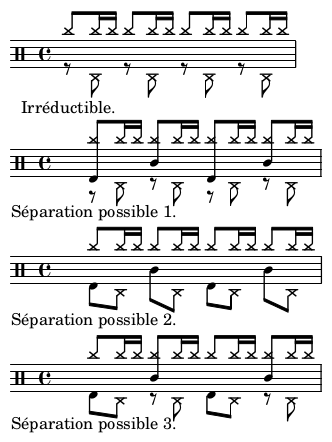
\includegraphics[height=60mm, width=40mm]{z_images/description_notation/separation/1_separation_4-4_binaire.png}\\\\
Ici, le système est construit sur un modèle rock en 4/4 : after-beat sur les 2 et 4 avec un choix de répartition des cymbales type fast-jazz. Le système est constitué par défaut du motif ride/ch-pf/cc et d’un texte joué à la grosse-caisse. La troisième séparation proposée est privilégiée car elle répartit selon 2 voix, une voix pour les mains (ride + cc) et une voix pour les pieds (ch-pf + gc). Ce choix paraît plus équilibré car deux instruments sont utilisés par voix et plus logique pour le lecteur puisque les mains sont en haut et les pieds en bas.\\
%D’autres choix d’écriture auraient été possibles :
%\begin{itemize}
%	\item Toutes les hampes en haut ;
%	\item Combinaison motif 1 et 2 en donnant 2 directions aux hampes de la cc).\\
%\end{itemize}

\textbf{Motif 4-4 jazz}\\\\
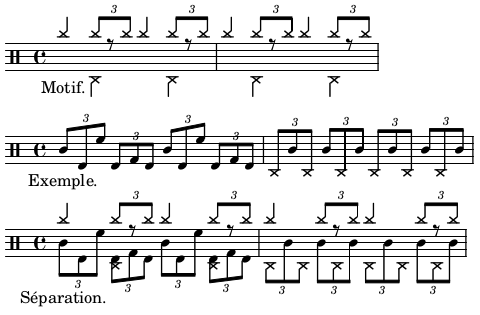
\includegraphics[height=45mm, width=60mm]{z_images/description_notation/separation/2_separation_4-4_jazz.png}\\\\
Dans la plupart des méthodes, le charley n’est pas écrit car considéré comme évident en jazz traditionnel. Ce qui facilite grandement l’écriture : la ride et les crash sur la voix du haut et le reste sur la voix du bas. Ici, le partie prit et de tout écrire. Dans l’exemple ci-dessus, les mesures 1 et 2 combinées avec le \textit{motif} de la première ligne, sont des cas typiques de la batterie jazz. Tout mettre sur la voix haute serait surchargé. De plus, la grosse caisse entre très souvent dans le flot des combinaisons de toms et de caisse claire et son écriture séparée serait inutilement compliquée et peu intuitive pour le lecteur. Le choix de séparation sera donc de laisser les cymbales en haut et toms, caisse-claire, grosse-caisse et pédale de charley en bas.\\

\textbf{Système 4-4 afro-cubain}\\\\
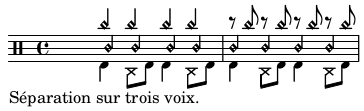
\includegraphics[height=25mm, width=80mm]{z_images/description_notation/separation/3_separation_afro-cubain.png}\\

\subsubsection{Pour la reconnaissance de la métrique}
\textit{\textbf{12/8 vs 4/4 ternaire}}\\\\
\textbf{Motif 12/8}\\\\
%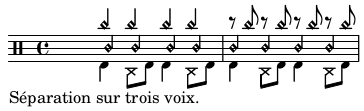
\includegraphics[height=30mm, width=100mm]{z_images/1_description_notation/separation/separation_2.png}\\\\

\subsubsection{Pour les règles de réécriture}
Les textes qui accompagnent les motifs étayent toutes les combinaisons d’un systèmes.\\


%\subsubsection{Construction des systèmes pour les expérimentations}
%\subsubsection{La réécriture des évènements MIDI pour la batterie}



\textbf{Exemples à écrire en arbre :}\\
\begin{itemize}
	\item 
	SI (pas pf) ET (note sur un temps suivie de note en l’air) :\\
	$\Rightarrow$ (Temps1 : Note pertinente) + (Temps2 : Silence pertinent + Note pertinente.)\\
	\item
	Si (po ou co) déborde sur le temps suivant :\\
	$\Rightarrow$ Liaison car marchera dans tous les cas même la où le point ne marchera pas (voir A2).\\
	\item
	Une blanche sera écrite noir + soupir.\\\\
\end{itemize}

%\newpage
%\subsubsection{Expérience 2}
%\textbf{Partition de référence pour l’ouput}
%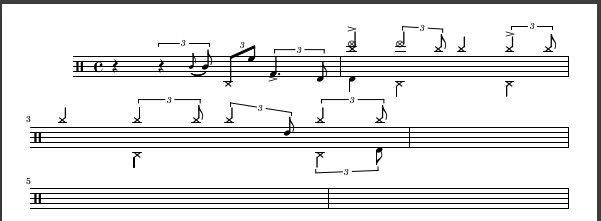
\includegraphics[height=50mm, width=160mm]{z_images/4_experimentations/experience_2/partition.png}\\\\
%\textit{En cours…}
\section*{Conclusion}
Bilan sur les différentes méthodes employées et la contribution que cela représente.